% main.tex
%=============================================================================
% Main document, including the IEEEtran preamble and content in one file

% Include the shared preamble
% Document class
\documentclass[conference,a4paper]{IEEEtran}

% Encoding and font
\usepackage[T1]{fontenc}
\usepackage[utf8]{inputenc}
\usepackage{lmodern}

% Graphics and paths
\usepackage{graphicx}
\graphicspath{{assets/images/}}
\usepackage{subcaption}

% Math packages
\usepackage{amsmath,amssymb}

% Hyperlinks
\usepackage[colorlinks=true, linkcolor=blue, urlcolor=blue, citecolor=blue]{hyperref}

% Color (for figures and highlights)
\usepackage{xcolor}

% Custom commands
% Example: Real numbers symbol
\newcommand{\R}{\mathbb{R}}

% Theorem environments (if needed)
\usepackage{amsthm}
\newtheorem{theorem}{Theorem}[section]
\newtheorem{lemma}[theorem]{Lemma}

\setlength{\marginparwidth}{2cm}
\usepackage{todonotes}
\usepackage{enumitem}
\usepackage{fancyhdr}

% Page layout adjustments (optional)
% \usepackage[margin=0.75in]{geometry}

% PDF metadata setup
\hypersetup{
  pdftitle    = {autowerkstatt4null: An Off-Board-Diagnostics Ecosystem for Car-Workshops},
  pdfauthor   = {Stephan Bökelmann, René Glitza, Gereon Kortenbruck, Lukas Jakubczyk, Meihui Huang, Odin Holmes},
  pdfsubject  = {Overview Paper for autowerkstatt4null},
  pdfkeywords = {AI diagnostics, federated learning, automotive workshops, oscilloscopes, GAIA-X, REST, WebSockets}
}


\begin{document}

% Title and Authors
\title{autowerkstatt4null: An Off-Board-Diagnostics Ecosystem for Car-Workshops}
\author{%
  \IEEEauthorblockN{%
    Stephan Bökelmann\IEEEauthorrefmark{1}, René Glitza\IEEEauthorrefmark{1},%
    Gereon Kortenbruck\IEEEauthorrefmark{2}, Lukas Jakubczyk\IEEEauthorrefmark{2},%
    Meihui Huang\IEEEauthorrefmark{3}, Odin Holmes\IEEEauthorrefmark{4}%
  }
  \IEEEauthorblockA{%
    \IEEEauthorrefmark{1}Ruhr University Bochum, Germany\\
    \IEEEauthorrefmark{2}THGA Bochum, Germany\\
    \IEEEauthorrefmark{3}nabla B engineering UG, Germany\\
    \IEEEauthorrefmark{4}Auto-Intern GmbH, Dortmund, Germany
  }
}

% Make the title area
\maketitle

% Abstract
\begin{abstract}
This paper presents Autowerkstatt 4.0, a three-year initiative funded by the German Federal Ministry for Economic Affairs and Climate Action to empower independent automotive workshops with AI-driven, federated diagnostics. 
We describe the current state of workshop diagnostics, the enabling technologies, our proposed ecosystem architecture, and initial user feedback. 
Key outcomes include a modular measurement platform, a secure data-exchange hub, asynchronous online diagnostics, and a learning academy for technician upskilling. 
Outlook includes integration of advanced AI modules and expanded federated capabilities.
\end{abstract}

% Keywords
\begin{IEEEkeywords}
AI diagnostics, federated learning, automotive workshops, oscilloscopes, GAIA-X, REST, WebSockets
\end{IEEEkeywords}

% 1. Introduction
\section{Introduction}
\subsection{State of Car Diagnostics}
\begin{figure}[ht]
  \centering
  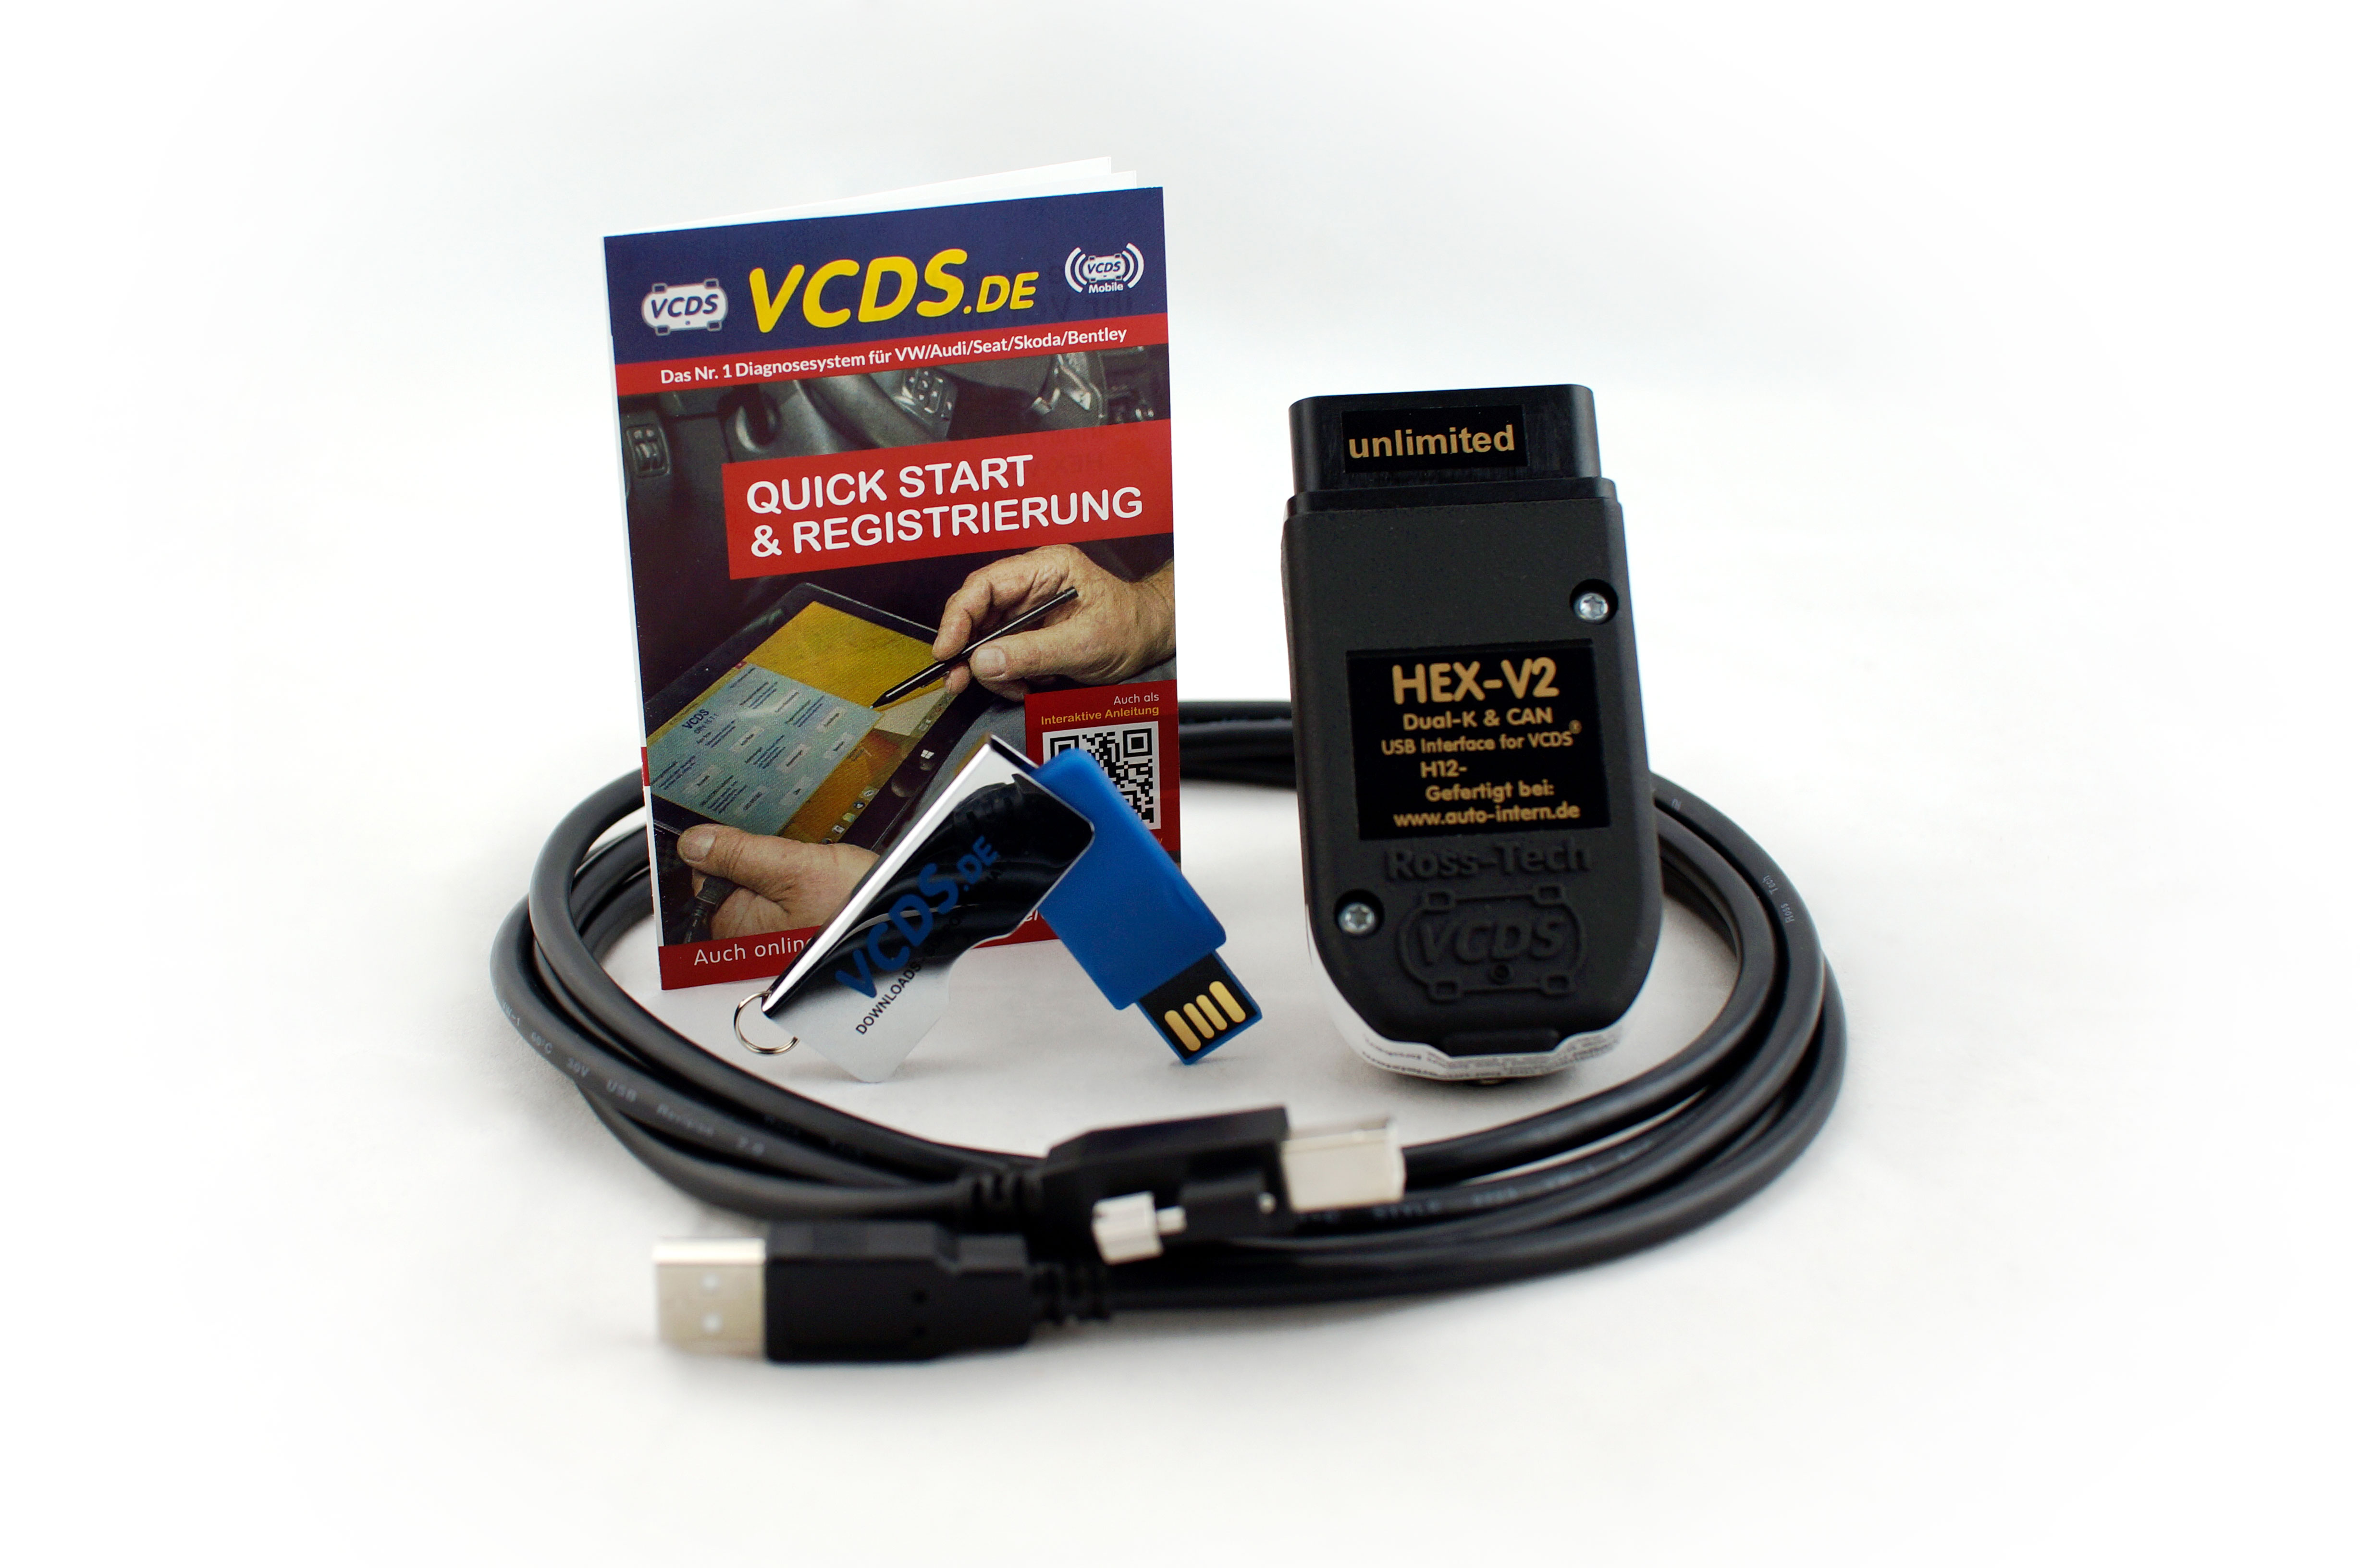
\includegraphics[width=0.8\linewidth]{obd_device}
  \caption{Picture of an OBD device}
  \label{fig:obd}
\end{figure}
Modern cars consist of a multitude of electronic, mechanic, and electromechanical subsystems. 
Market pressure and user demands regarding energy efficiency, comfort and passenger safety lead to an over-increasing complexity in the systems themselves and their interactions. 
Errorness behaviors in one of the subsystems can lead to various malfunctions. 
The purpose of car diagnostic systems is supporting technicians to identify the root cause of the malfunction.

Design goals for these car diagnostic systems are multiple:
-clarity and specificity of the erroneous part
-usability: easy to use correctly and hard to use incorrectly; teachability
-robustness against physical damage
-pricing
-costs of illformed diagnostics

Since some faults can lead to degraded combustion behaviors without noticeable effects for the car’s operator, some of these diagnostic systems have to be built into the car while others may reside in a sophisticated auto workshop, thus giving us the differentiation between on-board diagnostic and off-board diagnostic. 
According to this very definition, on-board diagnostic tools get delivered with each and every individual car itself, hence adding a) more costs; b) more weight; c) more complexity to the car.

It is therefore that auto manufacturers are trying to reduce the amount and extent of these systems to the least possible amount. 
Usually working against governmental regulations, the operators justified wish for the cars’ status information and the necessity to beware the cars’ systems to operate under potentially harmful conditions. 
In opposition to that, off-board systems do not need to be built into every car, but need to be bought by workshops. 
The market pressure for those tools arises out of the situation that mechanics get paid for maintaining and repairing a car but not necessarily the diagnostics itself. 
That’s why the evaluation of the cost-benefit ratios looks likely different for these tools.

\subsection{Future Challenges in ICEV and BEV}
Diversification in the set of cars also leads to a diversification in diagnostics. 
One particular fork in the road appears to be the further differentiation between internal combustion engine vehicles – ICEV; and battery electric vehicles – BEV. 
Both technologies confront auto shops with different diagnostic challenges. 
Yet both have in common that they include electrical signals and purely mechanical parts. 
While fault diagnostics of the purely mechanical parts of the car, e.g. suspension hinges, brakes, and fenders, can be categorized as a traditional craft, the diagnostics of peculiar electrical signals is as diverse as the ever-increasing amount of electrical assistant systems. 
A commonly used diagnostic tool for electrical fault analysis is the oscilloscope, which has been used in its traditional and auto shop specific variations by car technicians since the 1960s.

\subsection{Interesting Technologies for Upcoming Car Diagnostic Systems}
An oscilloscope is an electrical device with the purpose of projecting a time varying voltage (oscillation) onto a visible plane (scope), and with that displaying analytical features of the voltage visibly.

Working with oscilloscopes requires a certain depth of electrical understanding as well as proper handling of the necessary components, and well-trained pattern recognition of the recorded signals. 
These three qualities decrease the level of teachability significantly. 
Nevertheless, advanced electrical diagnosis requires recording timely varying voltages on an indicator of healthy or unhealthy behavior. 
Reiterating the previous argument about cost-benefit ratio of off-board diagnostic systems, this leads to a situation in which a useful tool cannot be trivially deployed to non-prepared auto shops, due to extensive learning curves.

Anyhow, we suspect to enhance teachability and robustness of these tools by employing certain technologies:
\begin{enumerate}[label=\alph*:) ]
  \item Machine Learning for Signal Clustering
  \item Modern Microcontroller Technology
  \item REST API \& Web Sockets
\end{enumerate}

\begin{figure}[ht]
  \centering
  \includegraphics[width=0.8\linewidth]{oscilloscopes}
  \caption{Three different Oscilloscopes}
  \label{fig:scopes}
\end{figure}
Review the role of high-speed waveform capture in pinpointing transient faults.

\subsubsection{Machine Learning for Signal Clustering}
\begin{figure}[ht]
  \centering
  \includegraphics[width=0.8\linewidth]{waveforms_good_bad}
  \caption{Two waveforms: a bad and a good measurement of a compression cycle}
  \label{fig:waveforms_good_bad}
\end{figure}
Programed computer functions can be understood as mappings of a domain to a codomain, where the domain is vulgarly referred to as input data and the codomain as output data. 
During the 1950s, researchers at Bell Laboratories and the Institute for Advanced Study in Princeton proposed that such programmatic functions could be executed autonomously by computer systems themselves 
— an idea that anticipated what is now formalized as the Universal Approximation Theorem Since then, this niche idea has evolved into a scientific discipline called Artificial Intelligence and Machine Learning. 
Latest advances in this area did demonstrate useful opportunities. 
It can thus be imagined to define an abstract function that maps a multidimensional time dependent vector of electrical quantities, also known as time series, to a certain fault category. 
From the toolkit of machine learning, multiple technologies could be interesting from a research stand point to generate such a function or group of functions, though all having in common a need for training data. 
The implementation of any of those functions could increase the specificity of fault identification while simultaneously decreasing the amount of training necessary for a mechanic to analyze signals.

\subsubsection{Modern Microcontroller Technology}
Traditional oscilloscopes usually come as all-in-one boxes, with high-accuracy analog front-ends and delicate signal processing units to display the measured voltages on a built-in screen. 
All of the mentioned parts are usually not meant for rough environments such as auto workshops. 
Specially designed electronic oscilloscopes that come in ruggedized cases may end up costing multiple thousands of euros.

So far, regular microcontrollers have not been used in oscilloscopes. 
However, recent generations of microcontrollers feature speeds that are high enough for sampling measurements in some auto shop use cases. 
In comparison to faster but also more expensive alternatives (e.g. FPGA, …), developing a sampling oscilloscope on a microcontroller basis with a USB interface to a regular computer, tablet, 
or smartphone could prove itself as a possible way forward for more robust yet inexpensive auto shop oscilloscopes.

\subsubsection{REST API and Web Sockets}
\begin{figure}[ht]
  \centering
  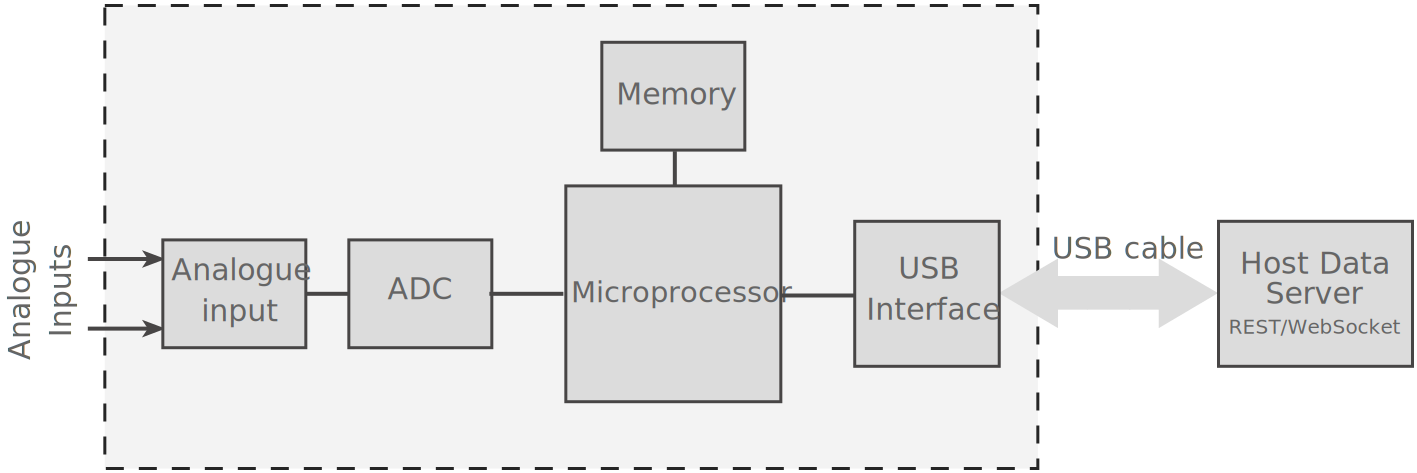
\includegraphics[width=0.8\linewidth]{data_server_architecture}
  \caption{Architecture diagram: scope connected to server via libusb and server providing REST/WebSocket}
  \label{fig:data-server}
\end{figure}
Since the two cornerstones — machine learning and microcontroller - based oscilloscopes — have been identified by now, the challenge of connecting them has to be addressed.

Since Machine Learning models require certain amounts of training data as well as centralized compute power, the according analysis models can be more easily run on centralized servers than on individual auto shop workstations. 
Yet, the data acquisition with the microcontroller oscilloscopes has to be performed on-site at the auto shop. 
Connecting these two modules could be done in a multitude of ways.

With the increasing employment of web technologies — especially HTTP (Hypertext Transfer Protocol)— it can be assumed that handling the data from acquisition to analysis could be implemented in an open-source approach. 
While doing that, the fundamental architecture needs to encompass two different modes of communication: asynchronous and synchronous.

\paragraph{Asynchronous Communication}
Asynchronous communication is not dependent on both ends of a communication channel having the same concept of time. 
This results in a certain pattern of communication that can also be described as a request–response model. 
One implementation using HTTP is REST (Representational State Transfer). 
These communication methods can be used to send a structured package of acquired data, including a recorded time series of a voltage as well as relevant metadata about this measurement, such as milage, sensor type, make-and-model of a car to a server’s interface called API. 
The server then has a certain amount of time to analyze the posted data, compare it against the internal database, formulate a response with a diagnosis and send it back to the requesting client.

\paragraph{Synchronous Communication}
The described pattern of analysis requires all of the posted data to be already in the RAM of the client’s machine, while the data itself can only be acquired one sample at a time over a certain period. 
Collecting these individual samples into a structured block necessitates that the computer’s input channel as well as the data collecting module run synchronously, meaning with the same idea of time. 
This can be done via an extension of the http called a web socket.

In conclusion this means that the middleware between USB-connected oscilloscopes and internet connected analysis service can be implemented using off-the-shelf web frameworks.

% 2. Proposed System
\section{Proposed System}
\subsection{Overview}
\begin{figure}[ht]
  \centering
  \includegraphics[width=0.8\linewidth]{system_architecture}
  \caption{Federated ecosystem architecture: data flow from scopes to AI services to technician UI}
  \label{fig:system_architecture}
\end{figure}
Provide a high-level overview of the federated ecosystem, showing secure data flows and component interactions.
Based on these previous considerations and the evergrowing complexity within cars, on-board-diagnostic solutions don't necessarily capture all the required use cases.
In this paragraph, a proposed off-board-diagnostic-solution is outlined, which might improve single car shops diagnostics capabilities by employing machine learning and data analytics.
Since the central entity of off-board diagnostics is ususally a techinician within a workshop, the first line of argumentation, that is entertained is their perspective on such a system.

\paragraph{Technician Workflow}
A customer's car enters a workshop. 
The first step taken in some cases is the full on-board-diagnostic scan resulting in a protocal of the quiry of all in the car available engine control units (abbr. ECU). 
This protocal encampsulates the status in which the car enters the workshop, compiling information such as milage, ECU series numbers, installed system with according hardware and software versions as well as potentially stored diagnostic trouble codes.
It is this protocal that can hint the technician to necessary maintenance or repair actions.
Unfortunately, due to the lack of sophistication of some of the on-board-diagnostic systems, DTCs don't always point out a problem in the most obvious way. 
An example for this is the diagnostic trouble code <DTC>
\todo[inline]{enter correct dtc here}
"Few pressure sensor output out of range" This DTC describes an invalid value arriving at the motor controller.
Even though it specifies a clear symptom, it does not yet contain information about the origin of that faulty behavior.
In stark contrast to what some people may think, diagnostic trouble codes do not directly indicate the necessary actions for repair.
After analyzing the set of trouble codes, a technician will always resort to differential diagnostics using off-board tools.
In case of the demostrated DTC, this might include validating the correct supply voltage to the sensor itself; 
validating the supply voltage to the motor control unit; validating the produced fuel pressure by utilizing an external pressure gauge; and validating the ohmic resistance of the signal line with a multi meter.
This differential diagnostic search tree is used and ordered to rule out one possible problem after another.
Depending on the read-out trouble codes, such a search tree might take up to hours or even days, resulting not only in a lenghty waiting process for the workshop's customer, but also hassle for the autoshop itself in terms of inner shop logistics.
In this very case, one single oscilloscope measurement measuring the signal on the line at the sensor connector and the motor controller connector could have been used to calculate the signal's transfer function $H(s)$ to rule out a whole plathora of electrical problems.
One of the reasons why this isn't done in autoshops lies in the mathematical complexity of this action itself as well as in non-existing data to compare the resulting transfer function to.
Using online services to store data to compare such values to and to calculate these functions out of time domain recordings could be an approach that takes the responsibility for the intellectual overhead.
By using a USB oscilloscope connected to a GUI program which presents the autoshop worker with clear instructions on how to attach the oscilloscope channels to specific signal lines in the car, sutomatically recording the data and sending it to a service is the key approach of this project. 
This proposed approach leads to multiple questions that need to be answered:
\item How can a GUI program support the technician workflow the best?
\item How can a low-cost yet rugged oscilloscope be manufactured in order to be rolled-out to the majority of workshops without introducing financial or usability barriers?
\item How can ever-improving analysis models be provided while simultaneously feeding back labled training data to algorithm developers?
\item Which data privacy aspects need to be considered for providing training data with high significance without opening malicious attack vectors?
\item How can training data be efficiently distributed to enable model developers to generate significant analysis models for the ever-growing variety of cars?

\subsection{Proof-of-Concepts}
Summarize laboratory and field tests demonstrating secure data exchange and basic AI inference.
In order to address these questions, the project aw4null aims to run proof of concept experiments.
Goals of these experiments are answering to the general fesability as well as to discover more detailed quetions.
The proposed system can be compartmentalized into the following fields:
\begin{enumerate} Use cases:
  \item hardware
  \item GUI usability
  \item data transport and sevice provisioning 
\end{enumerate}

\subsubsection{Data Transport and Provisioning}
In order for a produtive deployment of the proposed system, it must be figured out in what way acquired data from the workshop can be shared as a privacy preserving datum in a larger training data set, while also maintaining relevant meta information.
Not only does training data need to be shared but also models which were generated on this very training data set.
In succession of generating training data set and distilling analytical models, these models have to be distributed or provided as a service.

\paragraph{Side Note on Distributing or Provisioning of a Service}
Analytical models can be conceptualized as functions $Analysis = Model(Measurement)$.
This function needs to be evaluated on a machine.
Since it is expected that a model is not generated by a workshop, in a workshop, but rather by a signal conditioning expert that has no connection to the workshop, the measurement to be analyzed and the model to analyze with are stored on different machines.
This means that either the measurement data has to be sent to another machine on which the service function is available or the service function has to be transfered to the workshop machine prior to the actual diagnostic work. \hfill \\
In the demonstrator application different ideas to tackle this chanllenge shall be explored. 

\subsubsection{GUI Usability}
While developing a new diagnostic system, the ease of use can be a contributor to a project's success.
Auto-shop-technicians face an ever-increasing time- and efficiency- pressure, hence an efficient and effective user interface to all use-cases in the scope need to pass practical application tests inside real autoshops.
Furthermore, it must be made sure that the provided user-software is designed to be extended and forked without the necessity of refactoring.
Therefore, the aw4null project aims at an open-source-development for the demonstrator software.

\subsubsection{Hardware}
Automotive-oscilloscopes have been used for diagnostics since the 1970s already.
The market is saturaed, meaning that there are multiple options for each usecase available to the general autoshop.
Due to this, an evaluation of existing automotive-oscilloscopes shall be performed in order to find out whether or not availavle solutions meet the requirements of stirdiness, cost-benifit-ratio, and possibilities of intergration. \\

By proving a concept of intergration of these three layers, the project will outline a possible foundation for a next-generation off-board-diagnostics solution intergrating state-of-the-art electrical signal analysis and machine learning/artificial-intelligence capabilities.


\subsection{Demonstrator}
\begin{figure}[ht]
  \centering
  \includegraphics[width=0.8\linewidth]{early_scope}
  \caption{Early-Scope measurement prototype}
  \label{fig:early-scope}
\end{figure}

\begin{figure}[ht]
  \centering
  \includegraphics[width=0.8\linewidth]{old_gui_omniview}
  \caption{Legacy GUI: OmniView}
  \label{fig:gui}
\end{figure}

\begin{figure}[ht]
  \centering
  \includegraphics[width=0.8\linewidth]{data_api}
  \caption{Data gathering API interface}
  \label{fig:data-api}
\end{figure}
Detail the integrated pilot installation in partner workshops, including hardware setup and user interface snapshots.
The current demonstrator consists of six primary components:
\begin{itemize}
  \item A laptop equipped with OmniView and VCDS software
  \item A VCDS diagnostic tool
  \item Four OmniAIScopes
  \item Connection equipment (e.g., cables, Banana-to-BNC adapters)
  \item A formal contract
  \item Instructional materials
\end{itemize}
In accordance with the proposed workflow for car diagnostics, the process begins with connecting the vehicle to a VCDS device, which performs a standard OBD (on-board diagnostics) scan. 
As described in the Introduction, this step typically yields vague and sometimes insufficient error codes (DTCs), which are then displayed and recorded on the local laptop.

To improve diagnostic specificity, USB-based oscilloscopes—our OmniAIScopes—are connected to various electrical sensors in the vehicle using Banana-to-BNC adapters. 
Each scope records time-varying voltages from a specific sensor. 
These scopes are linked via a central hub, which aggregates signals and routes them to the local laptop, where the OmniView software allows real-time signal visualization and preliminary interpretation.

Collected measurement data is transferred via HTTP from the local hub to a remote web server. 
The web server then forwards the data to the central THGA server, where it is stored for future analysis. 
This architecture aligns with the proposed use of REST APIs for asynchronous communication and WebSockets for synchronous interaction, as described in the REST API and Web Sockets subsection of the introduction.

The long-term vision involves utilizing this stored signal data to train machine learning models capable of classifying faults based on signal patterns. 
However, due to the current lack of sufficient training data in the THGA repository, real-time diagnostic feedback based on these models is not yet operational. 
This aligns directly with the discussion in Machine Learning for Signal Clustering—highlighting the need for a significant and diverse training dataset before meaningful fault classification can be achieved.

The demonstrator has already been deployed in approximately 50–60 workshop environments over a six-month field test period, 
fulfilling the initial goals set out under the Proof-of-Concepts section in the proposed system. 
However, several challenges remain:
\begin{itemize}
  \item The various tools (VCDS, OmniView, hub interface, ML services) have not yet been unified into a single software platform, which limits usability.
  \item Training data volume remains insufficient, restricting the machine learning module’s ability to generate actionable feedback.
\end{itemize}



% 3. Results
\section{Results}
\subsection{Technical Readiness}
Report on system stability, latency, and throughput based on pilot metrics.

\subsection{Usage and Feedback}
Summarize technician survey results and adoption rates in participating workshops.

\subsection{Gathered Data}
Provide statistics on the volume, variety, and quality of collected waveform datasets.

% 4. Summary
\section{Summary}
Recap the key achievements: ecosystem architecture, live diagnostics, and workshop upskilling.

% 5. Outlook
\section{Outlook}
Discuss future work, including integration of the OmnAIScope platform, advanced federated ML modules, and expanded partner networks under GAIA-X.

\end{document}
